\documentclass[UTF8,a4paper,zihao=-4]{ctexart}

% ---------------------------------------------------------------------------
% Overleaf 编译说明
% ---------------------------------------------------------------------------
% 1. 上传本目录全部文件到 Overleaf。
% 2. Menu -> Compiler 选择 XeLaTeX。
% 3. main.tex 是主文件；正文由 body_content.tex 引入，图片位于 figures/。

\usepackage[a4paper,left=2.5cm,right=2.5cm,top=2.6cm,bottom=2.6cm]{geometry}
\usepackage{amsmath,amssymb}
\usepackage{graphicx}
\usepackage{booktabs}
\usepackage{longtable}
\usepackage{array}
\usepackage{calc}
\usepackage{float}
\usepackage{caption}
\usepackage{xcolor}
\usepackage{xurl}
\usepackage{hyperref}

\hypersetup{
  colorlinks=true,
  linkcolor=black,
  citecolor=black,
  urlcolor=blue
}

\graphicspath{{figures/}}
\setkeys{Gin}{width=0.92\linewidth,keepaspectratio}
\captionsetup[figure]{name=图,labelsep=quad,font=small}
\captionsetup[table]{name=表,labelsep=quad,font=small}

\setlength{\parindent}{2em}
\setlength{\parskip}{0.25em}
\linespread{1.25}
\emergencystretch=6em
\Urlmuskip=0mu plus 1mu

% Pandoc 生成正文时需要的兼容命令。
\providecommand{\tightlist}{%
  \setlength{\itemsep}{0pt}\setlength{\parskip}{0pt}}
\providecommand{\pandocbounded}[1]{#1}

\begin{document}

\begin{center}
  {\zihao{2}\heiti 基于 LSTM、Transformer 及其高效变体的长时序预测模型比较研究}\par
  \vspace{0.8em}
  {\zihao{4} 涂家俊\textsuperscript{1}}\par
  \vspace{0.3em}
  {\zihao{5}\textsuperscript{1} 合肥工业大学计算机与信息学院，合肥 230601}\par
\end{center}

\vspace{0.8em}

\noindent\textbf{摘\quad 要：}
长时序预测需要利用较长历史窗口对未来多个时间步进行连续预测，在能源负荷、交通流量、工业监测和气象分析等场景中具有重要应用价值。随着预测步长增加，模型不仅要捕捉局部趋势和周期变化，还需要面对长期依赖建模、误差累积和计算开销增大的问题。本文围绕 ETTh1 与 ETTm1 两个公开电力变压器温度数据集，比较 LSTM、Transformer、Informer、Autoformer 与 PatchTST 五类模型在多步预测任务中的表现。实验统一采用 96 步回看窗口，并设置 24、48、96、168、336 五种预测步长；评价指标包括 MSE、MAE、R$^2$ 与 MAPE，其中 MSE、MAE 和 R$^2$ 作为主要分析指标，MAPE 作为补充参考。本文以验证集最优配置重训得到的 v2 完整矩阵作为主实验结果，并进一步结合 v4 消融实验、完整单变量/多变量对比实验以及纯模型 forward 推理时间 benchmark，分析不同结构设计对预测精度、输入变量利用能力和计算效率的影响。实验结果表明，PatchTST 在 10 个数据集--预测步长任务中获得 9 次最低 MSE，整体性能最优；Autoformer 在部分高频序列任务上仍具有竞争力。消融结果显示，Autoformer 的序列分解模块和 PatchTST 的通道独立建模对性能贡献明显。单变量/多变量对比进一步说明，额外变量并不总能稳定改善目标列预测，能否抑制变量间噪声取决于模型结构。复杂度分析表明，PatchTST 在预测精度和纯 forward 推理效率之间表现出较好的平衡。

\vspace{0.4em}
\noindent\textbf{关键词：} 长时序预测；Transformer；PatchTST；Autoformer；消融实验；多变量预测

\vspace{0.4em}
\noindent\textbf{中图法分类号：} TP391.4

\vspace{1.4em}

\begin{center}
  {\zihao{3}\bfseries A Comparative Study of Long-term Time Series Forecasting Models Based on LSTM, Transformer and Efficient Variants}\par
  \vspace{0.8em}
  {\zihao{5} Tu Jiajun\textsuperscript{1}}\par
  \vspace{0.3em}
  {\zihao{5}\textsuperscript{1} School of Computer and Information, Hefei University of Technology, Hefei 230601, China}\par
\end{center}

\vspace{0.6em}

\noindent\textbf{Abstract:}
Long-term time series forecasting aims to predict multiple future time steps from historical observations and is widely used in energy, traffic and industrial monitoring scenarios. This paper compares five representative models, namely LSTM, Transformer, Informer, Autoformer and PatchTST, on the ETTh1 and ETTm1 datasets under a unified experimental setting. The look-back window is fixed to 96, and five forecasting horizons, 24, 48, 96, 168 and 336, are evaluated. The main results are based on the v2 full experiment matrix retrained with validation-selected configurations, while v4 ablation studies, univariate/multivariate comparisons and pure forward inference benchmarks are used for deeper analysis. The results show that PatchTST achieves the best overall accuracy and wins 9 out of 10 dataset-horizon tasks in terms of MSE. Ablation results further indicate that Autoformer's decomposition module and PatchTST's channel independence are important for performance. The univariate/multivariate comparison suggests that additional variables do not always improve target prediction unless the model can effectively reduce inter-variable noise. Efficiency analysis shows that PatchTST provides a favorable balance between forecasting accuracy and forward inference cost.

\vspace{0.4em}
\noindent\textbf{Key words:} long-term time series forecasting; Transformer; PatchTST; Autoformer; ablation study; multivariate forecasting

\newpage
\section{引言}\label{ux5f15ux8a00}

时间序列预测是机器学习与数据挖掘中的经典任务，目标是根据历史观测推断未来变化趋势。与单步预测相比，多步长时序预测更接近真实应用场景：在电力系统中，需要提前预测设备温度或负荷变化；在交通系统中，需要估计未来一段时间的流量波动；在工业监测中，则需要识别潜在异常趋势并提前安排维护。这类任务通常具有明显的周期性、趋势性和局部突变，并且预测步长越长，模型越容易受到未来不确定性和误差累积的影响。

传统循环神经网络能够顺序处理时间依赖，其中 LSTM 通过门控机制缓解普通 RNN 的梯度消失问题，在早期时序建模任务中应用广泛。然而，RNN 类模型的计算过程天然依赖时间步递推，并行能力有限；当输入窗口较长或预测步长较大时，模型可能难以稳定保留长距离信息。Transformer 通过自注意力机制增强了任意时间步之间的依赖建模能力，并具备更好的并行计算特性，但标准自注意力的计算复杂度随序列长度二次增长，直接用于长时序预测时可能带来较高计算开销，同时也未必能自动适配时间序列中的趋势和周期结构。

近年来，面向长时序预测的高效 Transformer 变体不断出现。Informer 通过 ProbSparse 注意力降低长序列注意力计算成本；Autoformer 引入序列分解和 Auto-Correlation 机制，将趋势项与季节项显式拆分；PatchTST 则将时间序列划分为 patch，并采用通道独立建模来降低变量间噪声干扰。这些方法从注意力稀疏化、周期结构建模和局部片段建模等不同角度改进了标准 Transformer，但在统一实验条件下，不同结构究竟如何影响预测精度和计算效率，仍需要通过系统实验加以比较。

本文围绕 ETTh1 与 ETTm1 两个 ETT 数据集开展实验，使用统一的数据划分、输入窗口、预测步长和评价指标比较 LSTM、Transformer、Informer、Autoformer 与 PatchTST 五种模型。本文的主要工作包括：（1）实现并比较 RNN 基线、标准 Transformer 及三类高效长时序 Transformer 变体；（2）基于验证集最优配置完成 2 个数据集、5 个预测步长、5 个模型共 50 组正式主实验；（3）通过调参前后对比、Autoformer/PatchTST 消融实验和单变量/多变量对比实验分析模型结构差异；（4）补充参数量、训练时间和纯模型 forward 推理时间，讨论预测性能与计算成本之间的权衡。

\section{相关工作}\label{ux76f8ux5173ux5de5ux4f5c}

\subsection{RNN 类时序预测模型}\label{rnn-ux7c7bux65f6ux5e8fux9884ux6d4bux6a21ux578b}

RNN 通过隐藏状态在时间维度上传递历史信息，适合处理顺序数据。LSTM 在 RNN 基础上引入输入门、遗忘门和输出门，使模型能够在一定程度上选择保留或遗忘历史信息，从而缓解梯度消失和长期依赖建模困难。对于中短期预测任务，LSTM 往往能够形成稳定的基线表现；但在长时序预测中，模型需要同时处理较长输入窗口和较长输出序列，递推式结构的并行效率不足，并且远期预测容易受到历史信息压缩和误差累积影响。因此，本文将 LSTM 作为 RNN 基线，用于衡量传统序列模型在统一任务设置下的性能下限。

\subsection{Transformer 与自注意力机制}\label{transformer-ux4e0eux81eaux6ce8ux610fux529bux673aux5236}

Transformer 使用自注意力机制直接建模任意位置之间的依赖关系，相比循环结构具有更强的并行计算能力。对于时间序列数据，自注意力可以在理论上捕捉远距离依赖，有助于处理长输入窗口。然而，标准自注意力的计算和存储复杂度通常为 \(O(L^2)\)，其中 \(L\) 为序列长度。当输入序列变长时，计算成本会迅速增加。此外，原始 Transformer 主要面向自然语言序列设计，并未显式建模时间序列常见的趋势、周期和多尺度局部模式。因此，直接将标准 Transformer 用于长时序预测，既可能面临效率问题，也可能在预测精度上弱于针对时序结构设计的专门模型。本文使用标准 Transformer 作为注意力机制基线，与后续高效变体进行比较。

\subsection{高效长时序预测模型}\label{ux9ad8ux6548ux957fux65f6ux5e8fux9884ux6d4bux6a21ux578b}

Informer 针对长序列预测中注意力计算成本过高的问题提出 ProbSparse 注意力，通过选择更有代表性的 query 减少无效注意力计算，并使用生成式解码方式一次性输出未来序列。Autoformer 则从时间序列结构出发，引入 series decomposition 将序列分为趋势项和季节项，并使用 Auto-Correlation 机制捕捉周期依赖，使模型更适合具有明显周期性的序列。PatchTST 的核心思想是将连续时间点划分为 patch，使模型在局部片段层面建模，同时采用 channel independence 将不同变量分别处理，减少多变量之间潜在噪声干扰。本文选择 Informer、Autoformer 和 PatchTST，是因为它们分别代表了注意力稀疏化、序列分解和 patch 化建模三类具有代表性的长时序预测思路。

\section{方法与实验设计}\label{ux65b9ux6cd5ux4e0eux5b9eux9a8cux8bbeux8ba1}

\subsection{任务定义}\label{ux4efbux52a1ux5b9aux4e49}

设多变量时间序列为 \(X=\{x_1,x_2,\ldots,x_T\}\)，其中每个时间步 \(x_t \in \mathbb{R}^{C}\)，\(C\) 为变量数。给定长度为 \(L\) 的历史窗口 \(X_{t-L+1:t}\)，模型需要预测未来 \(H\) 个时间步：

\[
\hat{Y}_{t+1:t+H}=f_{\theta}(X_{t-L+1:t})
\]

本文统一设置回看窗口 \(L=96\)，预测步长 \(H \in \{24,48,96,168,336\}\)。ETT 数据集中每个样本包含 7 个变量，因此多变量预测输入维度为 7。单变量实验中仅输入目标列并预测目标列；多变量实验中保留全部变量输入和输出，但比较时仍以目标列指标作为重点。

\subsection{数据集与预处理}\label{ux6570ux636eux96c6ux4e0eux9884ux5904ux7406}

本文使用 ETTh1 和 ETTm1 两个公开 ETT 数据集。ETTh1 为小时级采样数据，ETTm1 为 15 分钟级采样数据，二者均包含电力变压器相关变量，适合观察不同时间频率下的长步长预测表现。数据预处理遵循时间序列预测的基本要求：按照时间顺序划分训练集、验证集和测试集，避免未来信息泄露；使用训练集统计量进行标准化，并将相同变换应用于验证集和测试集；通过滑动窗口构造输入---输出样本，使所有模型在相同历史窗口和相同预测步长下训练与评估。

\subsection{模型设置}\label{ux6a21ux578bux8bbeux7f6e}

本文比较五类模型。为了让模型选择逻辑更清楚，表 1 先给出各模型在本文实验中的定位。LSTM 和 Transformer 分别作为 RNN 基线与标准注意力基线，Informer、Autoformer 和 PatchTST 则代表三类面向长时序预测的高效结构改进。

{\def\LTcaptype{none} % do not increment counter
\begin{longtable}[]{@{}
  >{\raggedright\arraybackslash}p{(\linewidth - 6\tabcolsep) * \real{0.2500}}
  >{\raggedright\arraybackslash}p{(\linewidth - 6\tabcolsep) * \real{0.2500}}
  >{\raggedright\arraybackslash}p{(\linewidth - 6\tabcolsep) * \real{0.2500}}
  >{\raggedright\arraybackslash}p{(\linewidth - 6\tabcolsep) * \real{0.2500}}@{}}
\toprule\noalign{}
\begin{minipage}[b]{\linewidth}\raggedright
模型
\end{minipage} & \begin{minipage}[b]{\linewidth}\raggedright
本文定位
\end{minipage} & \begin{minipage}[b]{\linewidth}\raggedright
关键思想
\end{minipage} & \begin{minipage}[b]{\linewidth}\raggedright
主要观察目的
\end{minipage} \\
\midrule\noalign{}
\endhead
\bottomrule\noalign{}
\endlastfoot
LSTM & RNN 基线 & 门控循环结构 & 检验传统序列模型在长步长预测中的下限表现 \\
Transformer & 标准注意力基线 & 全局自注意力 & 观察未专门适配时序结构的注意力模型表现 \\
Informer & 稀疏注意力变体 & ProbSparse attention & 分析降低长序列注意力开销后的预测表现 \\
Autoformer & 分解式长时序模型 & Series decomposition 与 Auto-Correlation & 验证趋势/季节分解对周期序列的作用 \\
PatchTST & Patch 化长时序模型 & Patching 与 channel independence & 分析局部片段建模和通道独立建模的效果 \\
\end{longtable}
}

为了保证比较公平，五个模型共享同一套数据接口、训练框架和评价指标。调参后的结构配置来自 ETTh1 h96 验证集最优实验，主要参数记录见 \texttt{docs/best\_model\_params.md}。表 2 列出本文 v2 主实验采用的模型结构参数；除特别说明外，各模型均使用 \texttt{dropout=0.1}。

{\def\LTcaptype{none} % do not increment counter
\begin{longtable}[]{@{}
  >{\raggedright\arraybackslash}p{(\linewidth - 2\tabcolsep) * \real{0.5000}}
  >{\raggedright\arraybackslash}p{(\linewidth - 2\tabcolsep) * \real{0.5000}}@{}}
\toprule\noalign{}
\begin{minipage}[b]{\linewidth}\raggedright
模型
\end{minipage} & \begin{minipage}[b]{\linewidth}\raggedright
结构参数
\end{minipage} \\
\midrule\noalign{}
\endhead
\bottomrule\noalign{}
\endlastfoot
LSTM & \texttt{hidden\_size=256}, \texttt{num\_layers=1} \\
Transformer & \texttt{d\_model=128}, \texttt{nhead=4}, \texttt{num\_layers=2}, \texttt{dim\_feedforward=128} \\
Informer & \texttt{d\_model=64}, \texttt{n\_heads=4}, \texttt{n\_encoder\_layers=2}, \texttt{n\_decoder\_layers=2}, \texttt{d\_ff=256}, \texttt{factor=3} \\
Autoformer & \texttt{d\_model=64}, \texttt{n\_heads=4}, \texttt{n\_encoder\_layers=2}, \texttt{n\_decoder\_layers=1}, \texttt{d\_ff=128}, \texttt{factor=3}, \texttt{kernel\_size=25} \\
PatchTST & \texttt{d\_model=64}, \texttt{n\_heads=8}, \texttt{n\_layers=2}, \texttt{d\_ff=128}, \texttt{patch\_len=32}, \texttt{stride=8} \\
\end{longtable}
}

\subsection{训练与调参设置}\label{ux8badux7ec3ux4e0eux8c03ux53c2ux8bbeux7f6e}

本文结果按版本组织。为避免读者混淆不同实验批次的用途，表 3 先说明本文涉及的主要结果版本。简言之，v1 用作未调参基线，v2 是正式主实验结果，v3 是单变量/多变量对比的阶段性验证，v4 则补齐消融实验和完整单变量/多变量分析。

{\small
\def\LTcaptype{none} % do not increment counter
\begin{longtable}[]{@{}
  >{\raggedright\arraybackslash}p{(\linewidth - 8\tabcolsep) * \real{0.1200}}
  >{\raggedright\arraybackslash}p{(\linewidth - 8\tabcolsep) * \real{0.1800}}
  >{\raggedright\arraybackslash}p{(\linewidth - 8\tabcolsep) * \real{0.2400}}
  >{\raggedright\arraybackslash}p{(\linewidth - 8\tabcolsep) * \real{0.2200}}
  >{\raggedright\arraybackslash}p{(\linewidth - 8\tabcolsep) * \real{0.2400}}@{}}
\toprule\noalign{}
\begin{minipage}[b]{\linewidth}\raggedright
版本
\end{minipage} & \begin{minipage}[b]{\linewidth}\raggedright
运行标签
\end{minipage} & \begin{minipage}[b]{\linewidth}\raggedright
数据范围
\end{minipage} & \begin{minipage}[b]{\linewidth}\raggedright
实验目的
\end{minipage} & \begin{minipage}[b]{\linewidth}\raggedright
本文用途
\end{minipage} \\
\midrule\noalign{}
\endhead
\bottomrule\noalign{}
\endlastfoot
v1 & 基线实验 & 2 数据集 × 5 步长 × 5 模型，共 50 组 & 使用未调参初始配置建立基线 & 只用于和 v2 比较调参前后变化 \\
v2 & 调优主实验 & 2 数据集 × 5 步长 × 5 模型，共 50 组 & 使用验证集最优配置重新训练完整矩阵 & 作为本文五模型性能比较的主结果 \\
v3 & 单/多变量预实验 & 2 数据集 × h96/h336 × 5 模型 × 2 输入模式，共 40 组 & 阶段性验证单变量/多变量实验流程 & 作为方法验证和历史归档，不作为正文主要结论来源 \\
v4 消融 & 结构消融实验 & 2 数据集 × h96/h336 × Autoformer/PatchTST 基线与消融变体，共 24 组 & 验证关键结构组件有效性 & 用于分析序列分解、通道独立等模块贡献 \\
v4 单/多变量 & 完整输入模式实验 & 2 数据集 × 5 步长 × 5 模型 × 2 输入模式，共 100 组 & 比较单变量和多变量输入对目标列预测的影响 & 用于分析额外变量是否稳定带来收益 \\
\end{longtable}
}

表中为便于阅读使用短标签；对应的原始运行标签分别为 \path{formal_seed42}、\path{full_val_best_e50p10_tb_seed42}、\path{feature_mode_full_seed42} 和 \path{ablation_rerun_seed42}。

v2 主实验统一使用 seed=42、batch size=128、最大训练轮数 50、early stopping patience=10。不同模型的学习率和权重衰减采用验证集调优结果，具体训练参数见表 4。测试集仅用于最终评估，不参与超参数选择。这样的设置避免了用测试集挑选模型带来的结果偏乐观问题，也使 v2 相比早期 v1 基线更适合作为最终性能比较口径。

{\def\LTcaptype{none} % do not increment counter
\begin{longtable}[]{@{}
  >{\raggedright\arraybackslash}p{(\linewidth - 12\tabcolsep) * \real{0.1111}}
  >{\raggedleft\arraybackslash}p{(\linewidth - 12\tabcolsep) * \real{0.1481}}
  >{\raggedleft\arraybackslash}p{(\linewidth - 12\tabcolsep) * \real{0.1481}}
  >{\raggedleft\arraybackslash}p{(\linewidth - 12\tabcolsep) * \real{0.1481}}
  >{\raggedleft\arraybackslash}p{(\linewidth - 12\tabcolsep) * \real{0.1481}}
  >{\raggedleft\arraybackslash}p{(\linewidth - 12\tabcolsep) * \real{0.1481}}
  >{\raggedleft\arraybackslash}p{(\linewidth - 12\tabcolsep) * \real{0.1481}}@{}}
\toprule\noalign{}
\begin{minipage}[b]{\linewidth}\raggedright
模型
\end{minipage} & \begin{minipage}[b]{\linewidth}\raggedleft
epochs
\end{minipage} & \begin{minipage}[b]{\linewidth}\raggedleft
patience
\end{minipage} & \begin{minipage}[b]{\linewidth}\raggedleft
batch size
\end{minipage} & \begin{minipage}[b]{\linewidth}\raggedleft
learning rate
\end{minipage} & \begin{minipage}[b]{\linewidth}\raggedleft
weight decay
\end{minipage} & \begin{minipage}[b]{\linewidth}\raggedleft
seed
\end{minipage} \\
\midrule\noalign{}
\endhead
\bottomrule\noalign{}
\endlastfoot
LSTM & 50 & 10 & 128 & 0.001 & 0.0 & 42 \\
Transformer & 50 & 10 & 128 & 0.0001 & 0.0 & 42 \\
Informer & 50 & 10 & 128 & 0.001 & 0.00001 & 42 \\
Autoformer & 50 & 10 & 128 & 0.001 & 0.00001 & 42 \\
PatchTST & 50 & 10 & 128 & 0.001 & 0.00001 & 42 \\
\end{longtable}
}

\subsection{评价指标与复杂度指标}\label{ux8bc4ux4ef7ux6307ux6807ux4e0eux590dux6742ux5ea6ux6307ux6807}

预测性能主要使用 MSE、MAE 和 R² 评价。MSE 对大误差更敏感，适合作为主排序指标；MAE 更直观地反映平均绝对偏差；R² 衡量模型相对均值预测基线的解释能力。MAPE 作为补充指标，但由于标准化后的时间序列中可能出现接近零的值，百分比误差容易被放大，因此本文不将 MAPE 作为唯一排序依据。

复杂度分析包含三类指标：模型参数量、训练时间和纯 forward 推理时间。参数量反映模型规模，训练时间反映训练成本，推理时间反映模型部署时单次前向计算成本。推理时间 benchmark 只测 \path{torch.inference_mode()} 下的 \path{model(x)}，不包含 DataLoader、数据搬运、反归一化、指标计算或结果保存时间。该 benchmark 在本机 Apple MPS 上完成，因此不能与 CUDA 训练时间直接混为同一硬件口径，只用于比较相同本机环境下的模型 forward 开销。

\section{实验结果与分析}\label{ux5b9eux9a8cux7ed3ux679cux4e0eux5206ux6790}

\subsection{五模型主实验结果}\label{ux4e94ux6a21ux578bux4e3bux5b9eux9a8cux7ed3ux679c}

v2 主实验结果显示，PatchTST 在整体平均 MSE 上表现最好。跨 ETTh1、ETTm1 和五个预测步长取平均后，PatchTST 的平均 MSE 为 0.462621，Autoformer 为 0.501605，Transformer 为 0.821683，Informer 为 0.890119，LSTM 为 0.987132。目标列指标也呈现类似趋势：PatchTST 的平均 \texttt{MSE\_target} 为 0.077168，Autoformer 为 0.094870，明显优于其余模型。按 10 个数据集---预测步长任务统计，PatchTST 获得 9 次最低 MSE，Autoformer 获得 1 次最低 MSE。

表 5 汇总了 v2 主实验中五个模型跨 10 个任务的平均表现。可以看到，PatchTST 在 MSE、MAE、R² 和目标列 MSE 上均排名最优，Autoformer 排名第二；LSTM 参数量最高，但误差也最高，说明模型规模并不能直接转化为预测性能。

{\def\LTcaptype{none} % do not increment counter
\begin{longtable}[]{@{}
  >{\raggedright\arraybackslash}p{(\linewidth - 12\tabcolsep) * \real{0.1111}}
  >{\raggedleft\arraybackslash}p{(\linewidth - 12\tabcolsep) * \real{0.1481}}
  >{\raggedleft\arraybackslash}p{(\linewidth - 12\tabcolsep) * \real{0.1481}}
  >{\raggedleft\arraybackslash}p{(\linewidth - 12\tabcolsep) * \real{0.1481}}
  >{\raggedleft\arraybackslash}p{(\linewidth - 12\tabcolsep) * \real{0.1481}}
  >{\raggedleft\arraybackslash}p{(\linewidth - 12\tabcolsep) * \real{0.1481}}
  >{\raggedleft\arraybackslash}p{(\linewidth - 12\tabcolsep) * \real{0.1481}}@{}}
\toprule\noalign{}
\begin{minipage}[b]{\linewidth}\raggedright
模型
\end{minipage} & \begin{minipage}[b]{\linewidth}\raggedleft
平均 MSE
\end{minipage} & \begin{minipage}[b]{\linewidth}\raggedleft
平均 MAE
\end{minipage} & \begin{minipage}[b]{\linewidth}\raggedleft
平均 R²
\end{minipage} & \begin{minipage}[b]{\linewidth}\raggedleft
目标列 MSE
\end{minipage} & \begin{minipage}[b]{\linewidth}\raggedleft
平均参数量
\end{minipage} & \begin{minipage}[b]{\linewidth}\raggedleft
平均训练时间/s
\end{minipage} \\
\midrule\noalign{}
\endhead
\bottomrule\noalign{}
\endlastfoot
PatchTST & 0.4626 & 0.4497 & 0.6366 & 0.0772 & 113037 & 58.7 \\
Autoformer & 0.5016 & 0.4779 & 0.6061 & 0.0949 & 110689 & 88.3 \\
Transformer & 0.8217 & 0.6740 & 0.3547 & 0.3736 & 338067 & 82.6 \\
Informer & 0.8901 & 0.6860 & 0.3010 & 0.5254 & 192884 & 67.1 \\
LSTM & 0.9871 & 0.6998 & 0.2249 & 0.2651 & 578938 & 41.1 \\
\end{longtable}
}

\begin{figure}
\centering
\pandocbounded{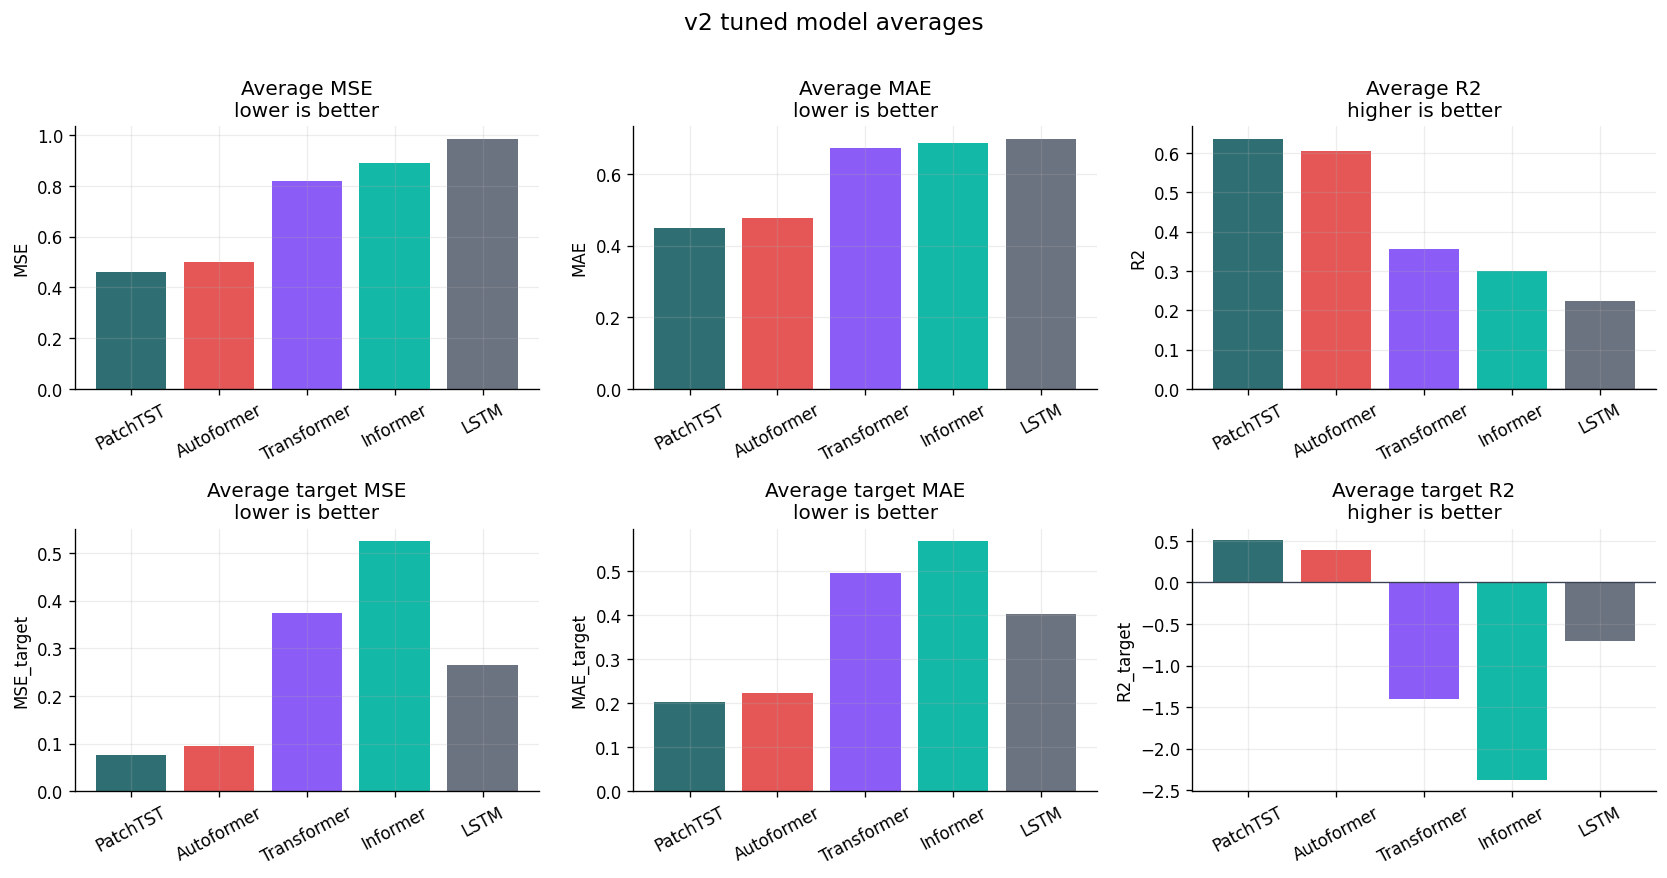
\includegraphics[keepaspectratio]{figures/v2_model_average_metrics.png}}
\caption{v2 五模型平均指标}
\end{figure}

从预测步长趋势看，随着 horizon 从 24 增加到 336，多数模型误差上升、R² 下降，说明长步长预测确实存在更明显的不确定性和误差累积。PatchTST 在多数任务上保持最低误差，可能与其 patch 化输入方式有关：连续时间点被组织成局部片段后，模型能在较短 token 序列上捕捉局部形态，同时保留长窗口中的整体变化。Autoformer 的表现也较稳定，说明序列分解对于 ETT 这类具有趋势和周期结构的数据有实际作用。

\begin{figure}
\centering
\pandocbounded{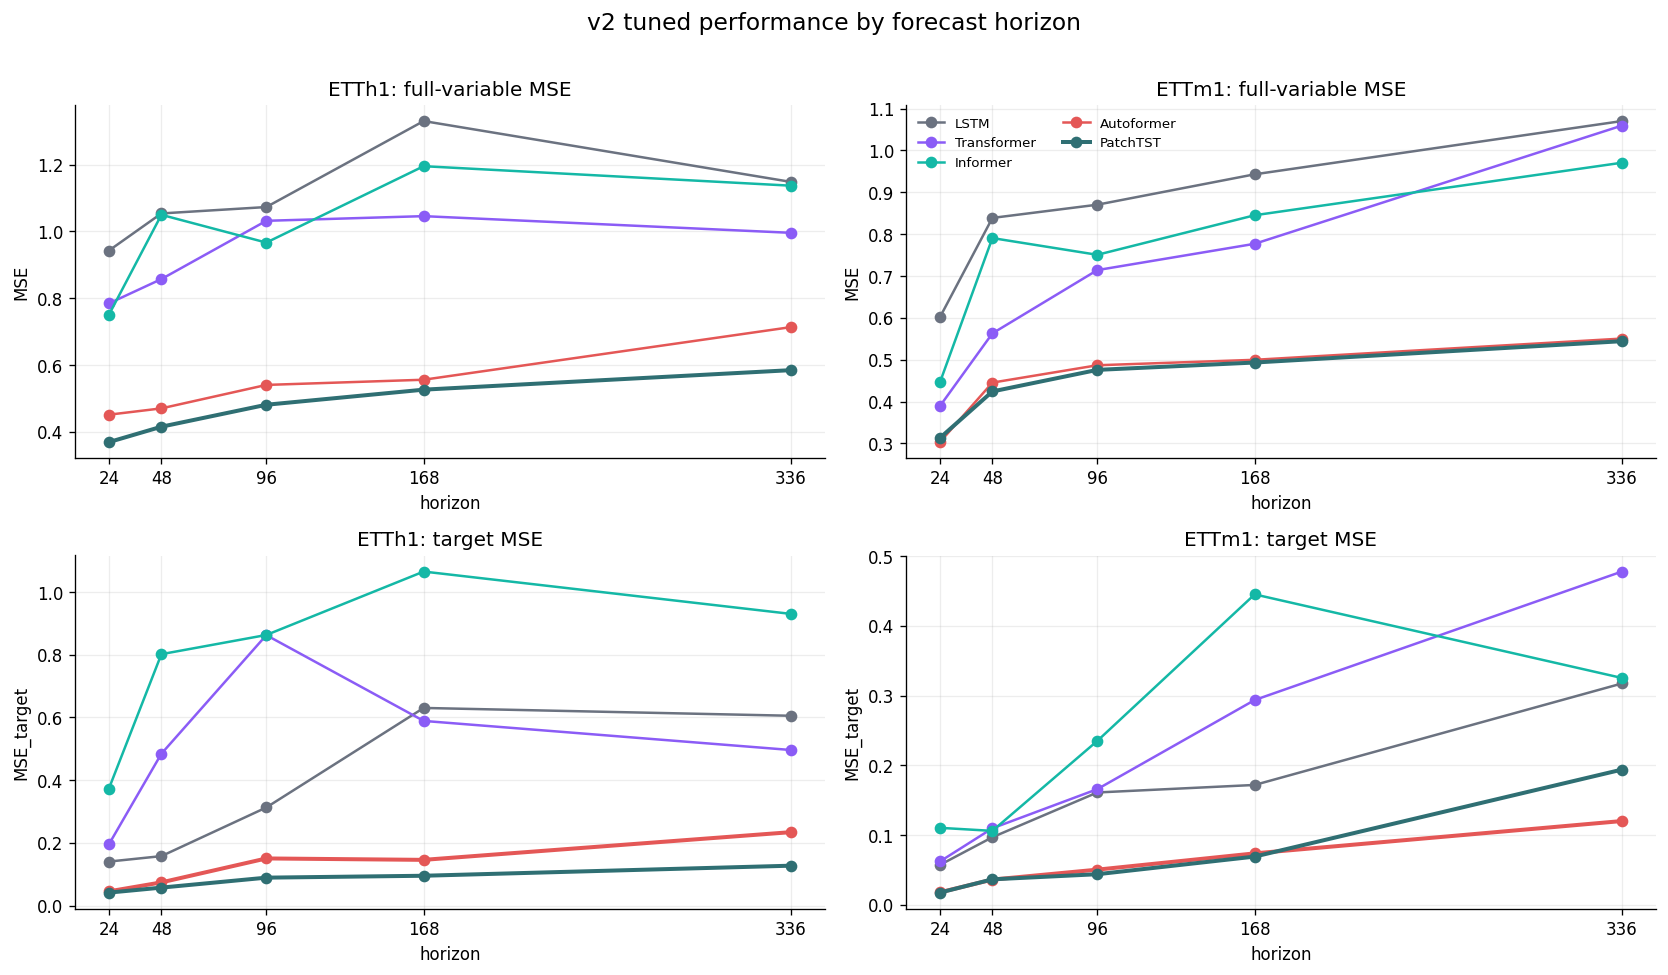
\includegraphics[keepaspectratio]{figures/v2_horizon_trends.png}}
\caption{v2 不同预测步长趋势}
\end{figure}

\begin{figure}
\centering
\pandocbounded{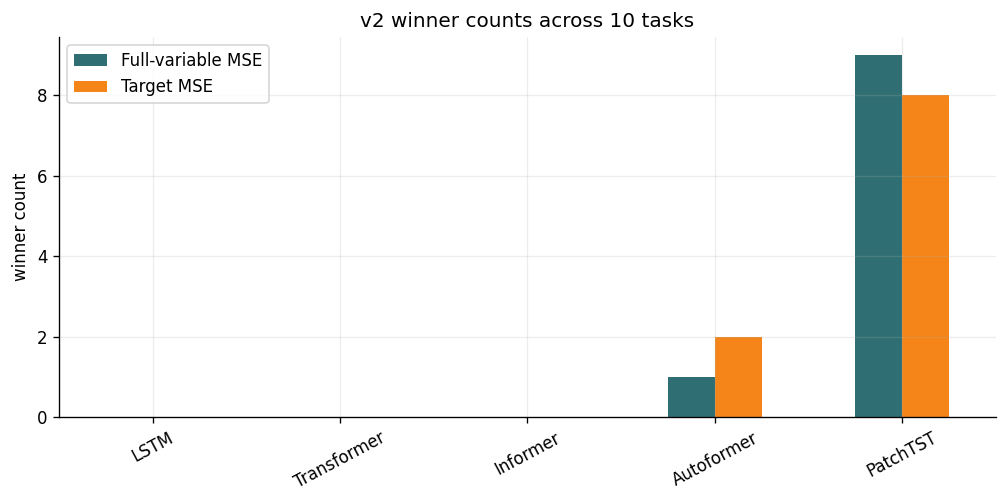
\includegraphics[keepaspectratio]{figures/v2_winner_counts.png}}
\caption{v2 任务胜出次数}
\end{figure}

LSTM 与标准 Transformer 的表现整体弱于 Autoformer 和 PatchTST。LSTM 的平均参数量较高，但平均 MSE 最高，说明仅增加循环结构规模不能充分解决长步长预测问题。标准 Transformer 虽然具备全局注意力建模能力，但没有显式处理时序趋势、周期和多变量干扰，因此在本实验中未能超过面向长时序设计的模型。

\subsection{调参前后对比}\label{ux8c03ux53c2ux524dux540eux5bf9ux6bd4}

v1 未调参基线用于观察初始配置下模型表现，v2 则使用验证集最优配置重训。对比结果显示，Transformer 调参收益最明显，平均 MSE 从 0.917 降至 0.822，约下降 10.4\%；Autoformer 从 0.515 降至 0.502，约下降 2.5\%；PatchTST 从 0.469 降至 0.463，约下降 1.4\%。这说明验证集调参对不同模型的影响并不一致：结构本身已经较适配任务的模型提升空间较小，而对超参数更敏感的模型则可能明显受益。

表 6 进一步给出 v1 与 v2 的平均 MSE 对比。变化率按 \((v2-v1)/v1\) 计算，因此负值表示调参后误差下降，正值表示调参后平均误差上升。

{\def\LTcaptype{none} % do not increment counter
\begin{longtable}[]{@{}lrrr@{}}
\toprule\noalign{}
模型 & v1 平均 MSE & v2 平均 MSE & MSE 变化率/\% \\
\midrule\noalign{}
\endhead
\bottomrule\noalign{}
\endlastfoot
PatchTST & 0.4693 & 0.4626 & -1.4 \\
Autoformer & 0.5147 & 0.5016 & -2.5 \\
Transformer & 0.9173 & 0.8217 & -10.4 \\
Informer & 0.8170 & 0.8901 & 8.9 \\
LSTM & 0.9461 & 0.9871 & 4.3 \\
\end{longtable}
}

\begin{figure}
\centering
\pandocbounded{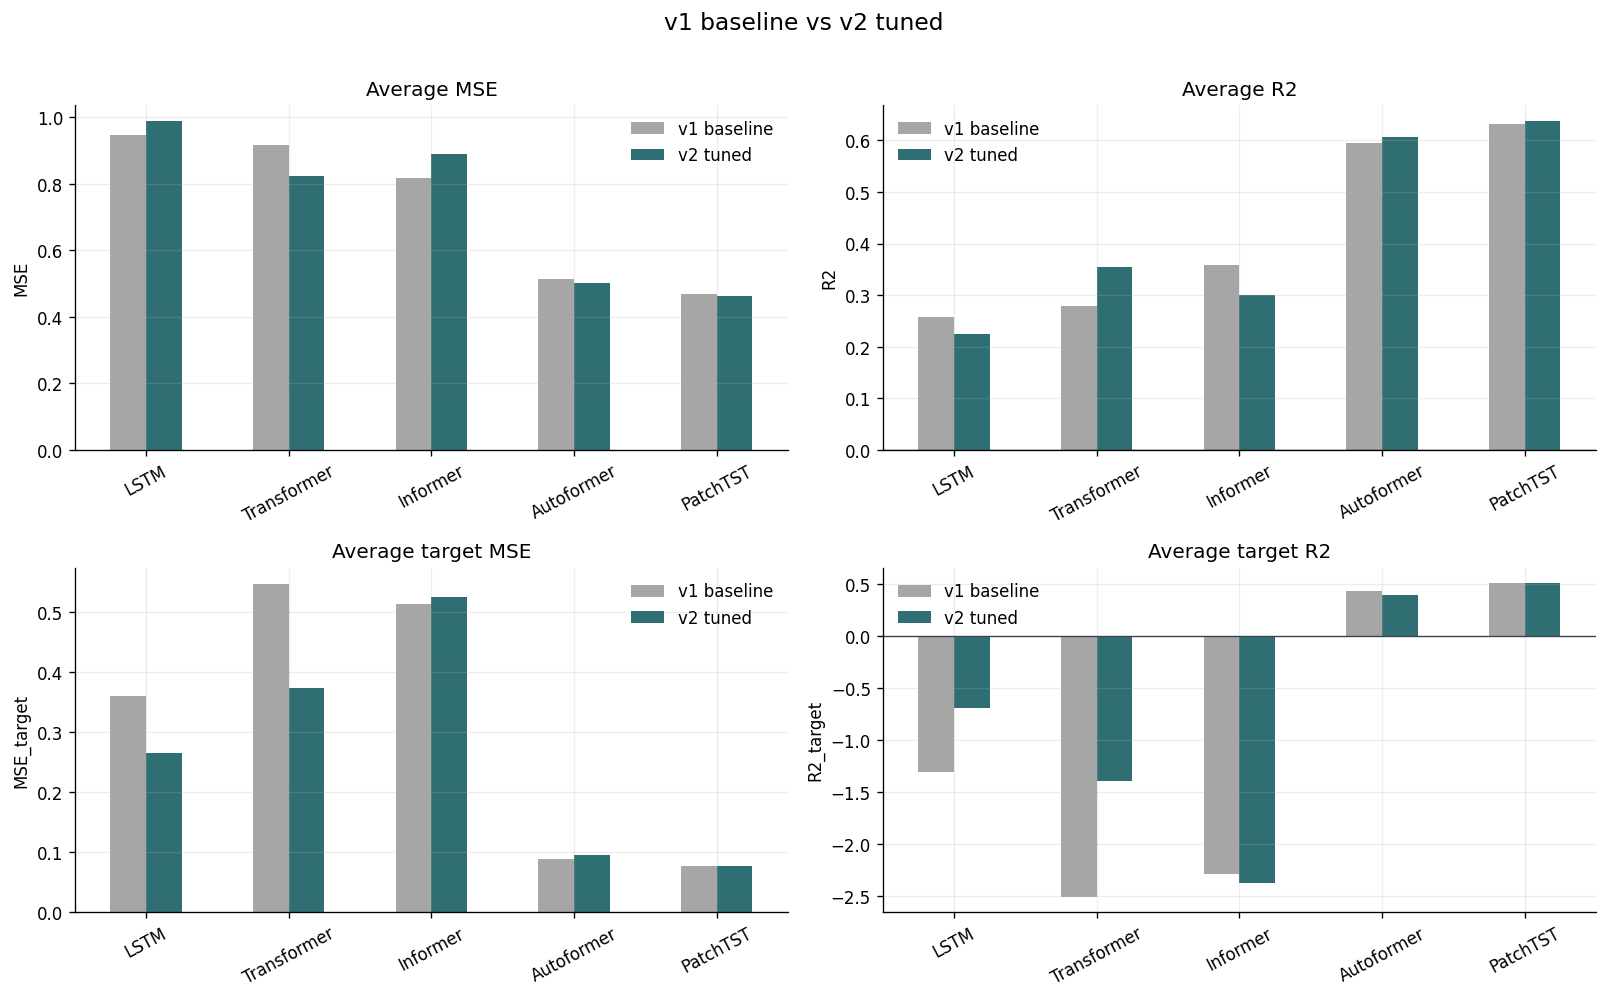
\includegraphics[keepaspectratio]{figures/v2_vs_v1_model_comparison.png}}
\caption{v2 与 v1 模型平均表现对比}
\end{figure}

也需要看到，Informer 和 LSTM 在 v2 平均 MSE 上相对 v1 并未提升。该现象说明``验证集最优配置''并不必然带来所有测试任务的平均改善，尤其当调参依据来自特定数据集和特定步长时，配置迁移到其他数据集或预测步长后可能存在泛化差异。因此，本文将 v2 作为主结果，并不是因为它在每个模型上都优于 v1，而是因为 v2 的选择过程更规范：先由验证集确定配置，再统一在测试集上报告最终结果。

\begin{figure}
\centering
\pandocbounded{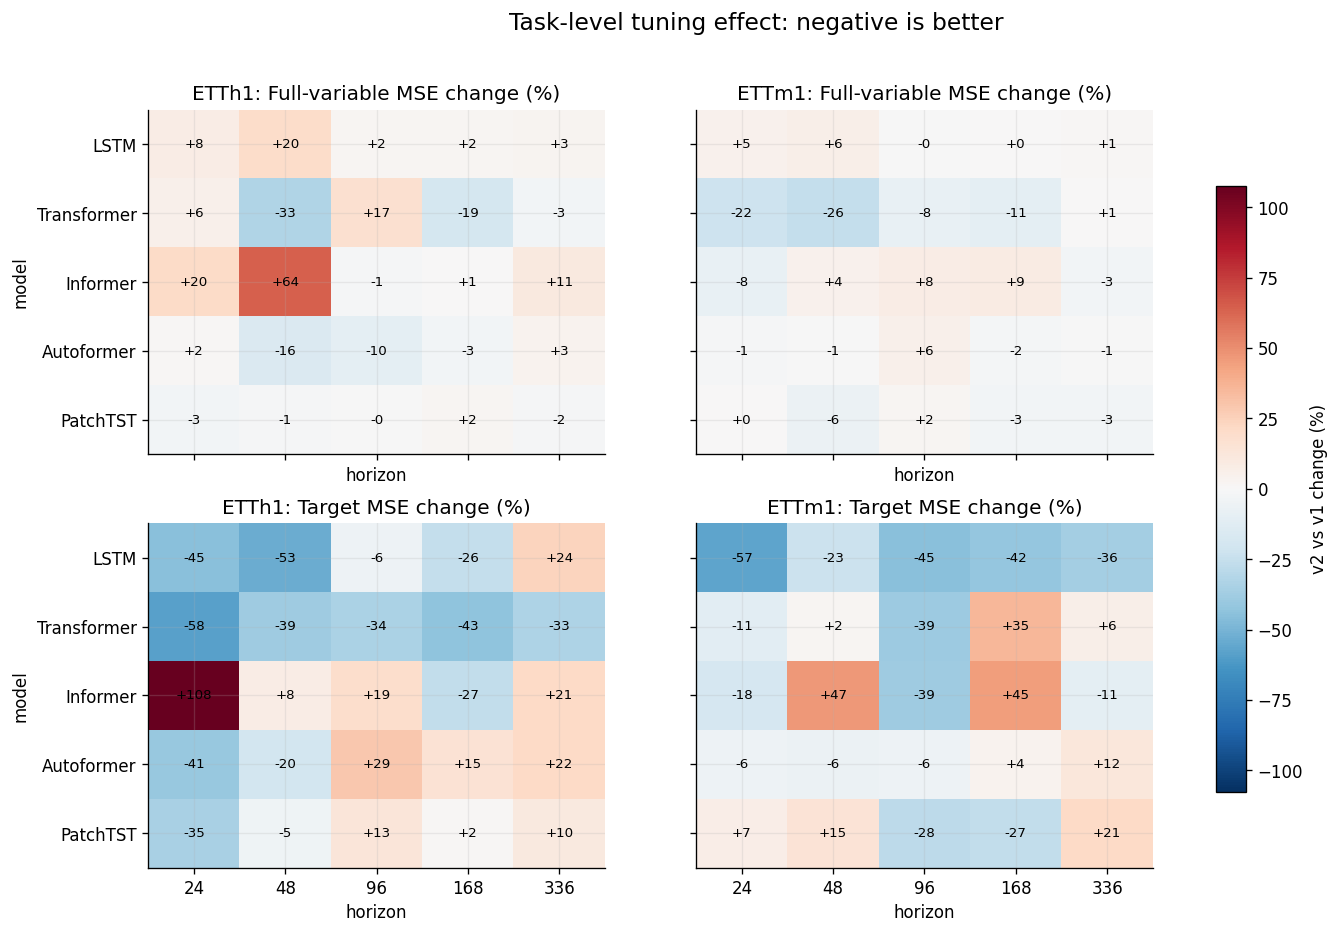
\includegraphics[keepaspectratio]{figures/v2_vs_v1_task_improvement_heatmap.png}}
\caption{v2 相对 v1 的逐任务变化热力图}
\end{figure}

\subsection{消融实验}\label{ux6d88ux878dux5b9eux9a8c}

为分析关键结构的有效性，本文使用 v4 消融实验比较 Autoformer 和 PatchTST 的基线版本与结构变体。消融范围覆盖 ETTh1、ETTm1 的 h96 和 h336，每个模型包含同批次基线和对应消融变体。结果表明，Autoformer 去掉序列分解模块后，平均 MSE 增加 0.386531，平均相对上升约 66.2\%，R² 平均下降 0.304086。这说明 series decomposition 对 Autoformer 的预测性能具有明显贡献，尤其在含有趋势和周期结构的 ETT 数据中，显式拆分趋势项和季节项能够降低模型直接学习复杂混合模式的难度。

表 7 汇总了四类消融变体相对同批次基线的平均变化。\texttt{mean\_delta\_MSE\_pct} 为正表示移除或替换组件后 MSE 上升，即性能退化；为负则表示消融版本在当前实验平均值上略优。

{\small
\def\LTcaptype{none} % do not increment counter
\begin{longtable}[]{@{}
  >{\raggedright\arraybackslash}p{(\linewidth - 8\tabcolsep) * \real{0.2200}}
  >{\raggedright\arraybackslash}p{(\linewidth - 8\tabcolsep) * \real{0.2400}}
  >{\raggedleft\arraybackslash}p{(\linewidth - 8\tabcolsep) * \real{0.1700}}
  >{\raggedleft\arraybackslash}p{(\linewidth - 8\tabcolsep) * \real{0.1900}}
  >{\raggedleft\arraybackslash}p{(\linewidth - 8\tabcolsep) * \real{0.1800}}@{}}
\toprule\noalign{}
\begin{minipage}[b]{\linewidth}\raggedright
基线模型
\end{minipage} & \begin{minipage}[b]{\linewidth}\raggedright
消融模型
\end{minipage} & \begin{minipage}[b]{\linewidth}\raggedleft
平均 ΔMSE
\end{minipage} & \begin{minipage}[b]{\linewidth}\raggedleft
平均 ΔMSE/\%
\end{minipage} & \begin{minipage}[b]{\linewidth}\raggedleft
平均 ΔR²
\end{minipage} \\
\midrule\noalign{}
\endhead
\bottomrule\noalign{}
\endlastfoot
Autoformer 基线 & 去 Auto-Correlation & -0.0207 & -3.1 & 0.0163 \\
Autoformer 基线 & 去序列分解 & 0.3865 & 66.2 & -0.3041 \\
PatchTST 基线 & 通道混合 & 0.7212 & 139.2 & -0.5665 \\
PatchTST 基线 & 去 patch 化 & 0.0388 & 7.7 & -0.0305 \\
\end{longtable}
}

\begin{figure}
\centering
\pandocbounded{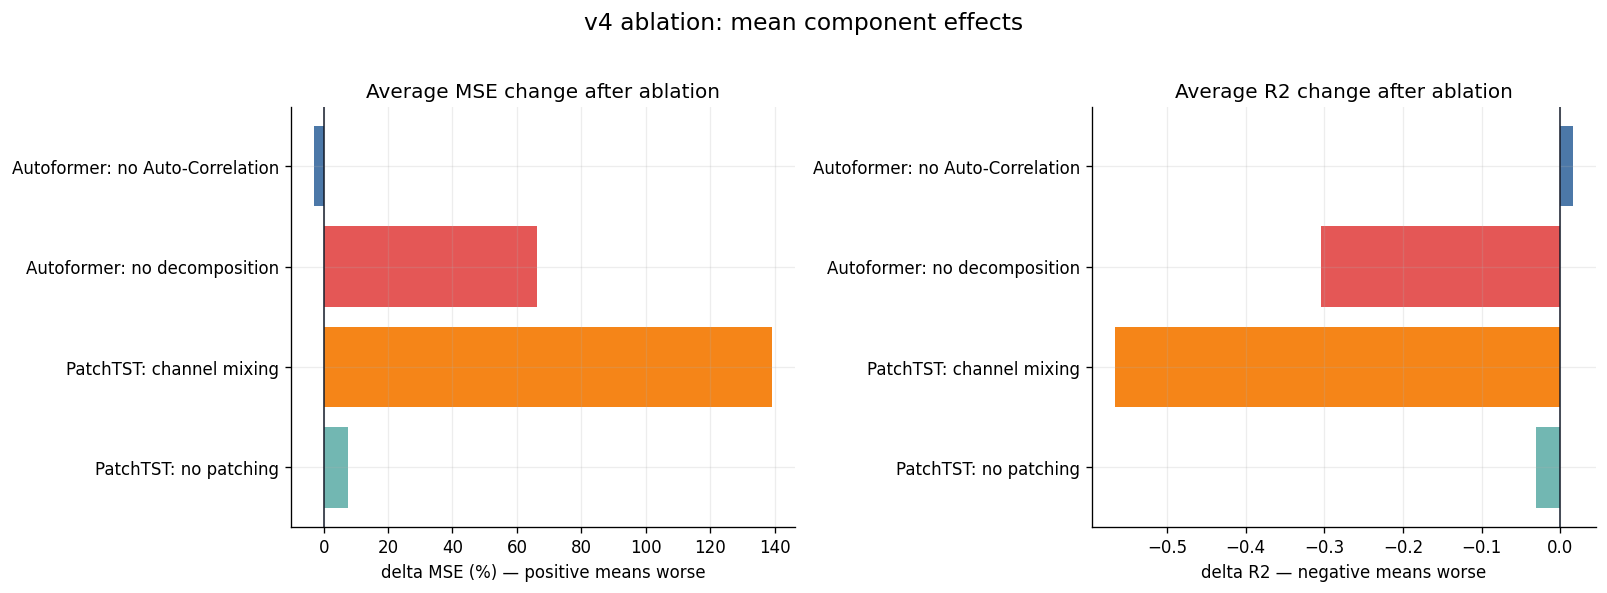
\includegraphics[keepaspectratio]{figures/v4_ablation_mean_effects.png}}
\caption{v4 消融平均影响}
\end{figure}

PatchTST 的消融结果同样明显。取消 channel independence 后，平均 MSE 增加 0.721228，平均相对上升约 139.2\%，R² 平均下降 0.566507。这表明通道独立建模是 PatchTST 在当前实验中最关键的结构之一。对于多变量时间序列，不同变量之间并非总是提供有效互补信息，直接混合所有变量可能引入噪声；PatchTST 分通道建模后再共享预测结构，能够在保留单变量模式的同时减少变量间干扰。

\begin{figure}
\centering
\pandocbounded{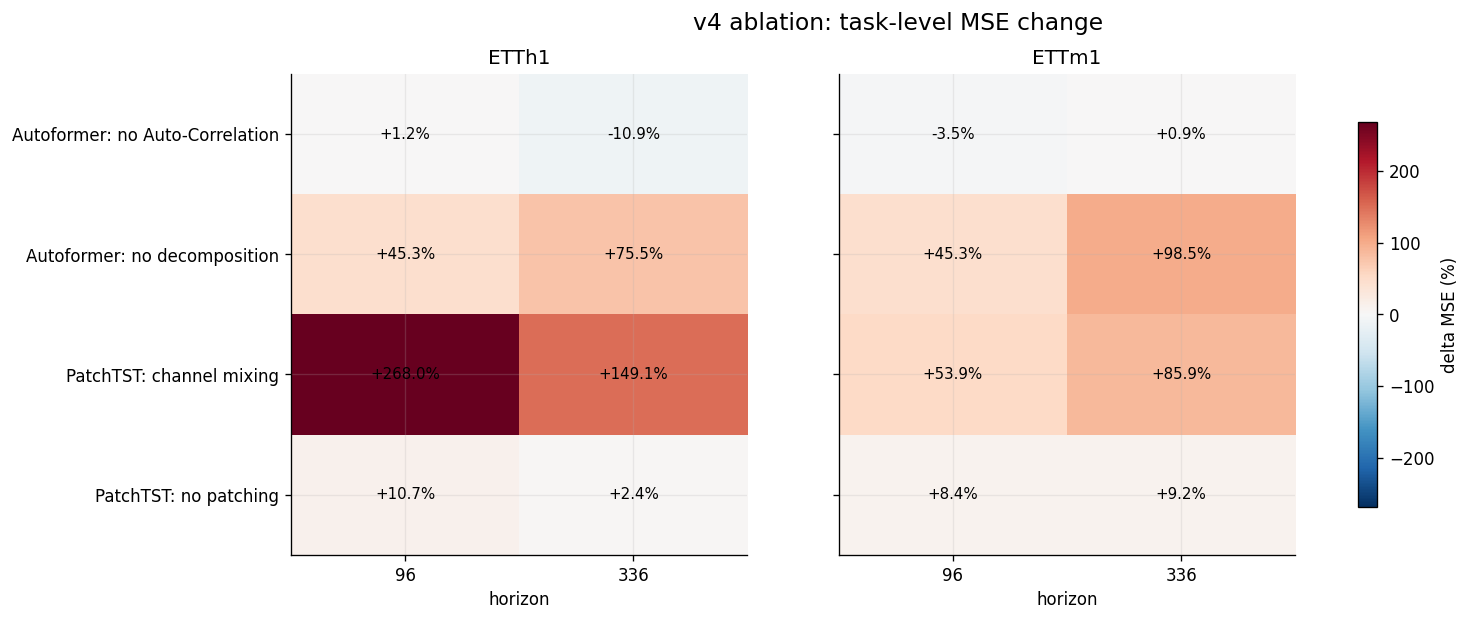
\includegraphics[keepaspectratio]{figures/v4_ablation_task_delta_heatmap.png}}
\caption{v4 消融逐任务热力图}
\end{figure}

相比之下，将 Autoformer 的 Auto-Correlation 替换为标准注意力后，平均 MSE 变化为 -0.020742，即部分任务中消融版本反而略好。这一结果不能简单理解为 Auto-Correlation 无效，更可能与本文中的轻量实现、数据规模、训练预算和超参数选择有关。Auto-Correlation 的优势通常依赖更充分的周期性建模和合适的结构规模；在课程项目的轻量实现中，该模块可能尚未完全发挥原论文设定下的效果。因此，本文对该项消融采取谨慎解释：序列分解和通道独立的贡献非常明确，而 Auto-Correlation 的贡献还需要更系统的超参数与多随机种子实验验证。

\begin{figure}
\centering
\pandocbounded{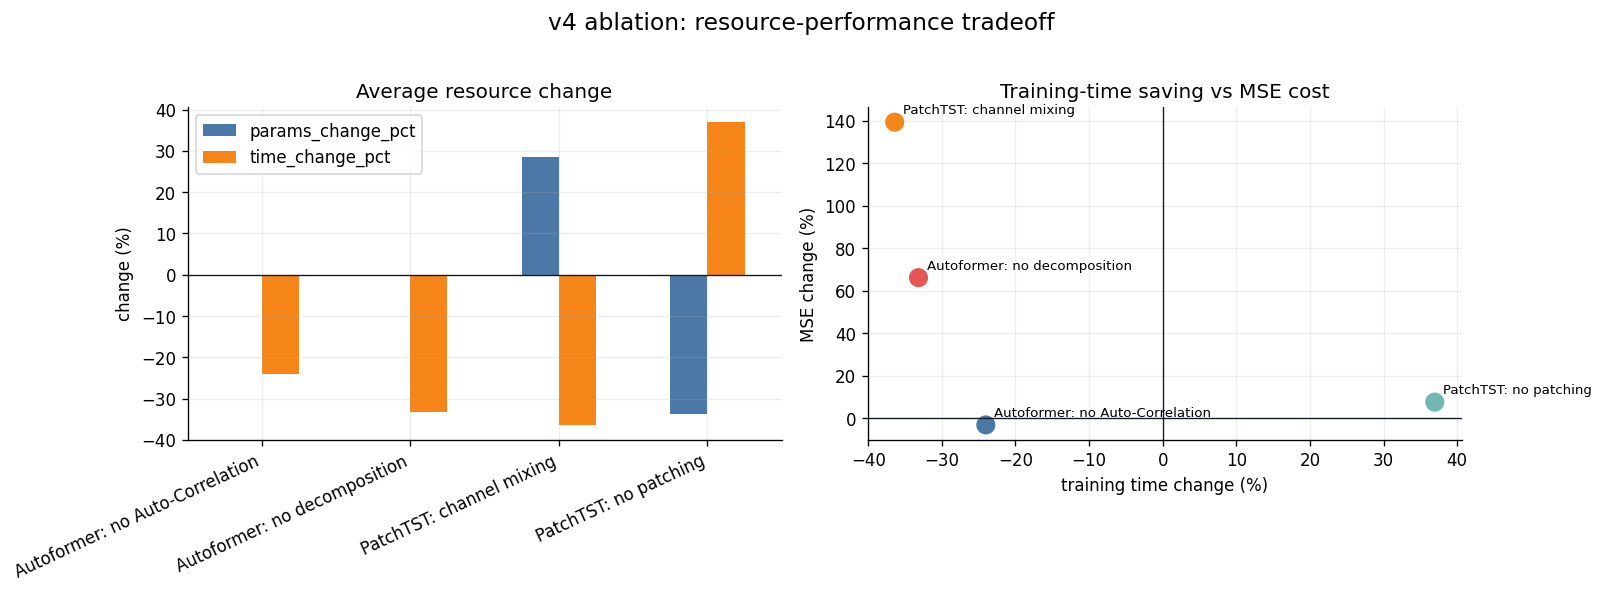
\includegraphics[keepaspectratio]{figures/v4_ablation_resource_tradeoff.png}}
\caption{v4 消融资源与性能权衡}
\end{figure}

\subsection{单变量与多变量对比}\label{ux5355ux53d8ux91cfux4e0eux591aux53d8ux91cfux5bf9ux6bd4}

多变量预测通常被认为可以利用额外变量提供的信息，但额外变量也可能带来噪声和优化难度。v4 单变量/多变量完整对比覆盖 ETTh1、ETTm1、五个预测步长、五个模型和两种输入模式，共 100 组实验，并形成 50 个严格配对任务。结果显示，在目标列 MSE 上，单变量模式赢得 43 个配对任务，多变量模式赢得 7 个任务；这 7 次多变量优势全部来自 PatchTST。

表 8 按模型统计了 10 个数据集---预测步长任务中单变量和多变量模式的胜出次数。除 PatchTST 外，其余四个模型均为单变量模式 10 次胜出；PatchTST 则有 7 次由多变量模式取得更低目标列 MSE。

{\def\LTcaptype{none} % do not increment counter
\begin{longtable}[]{@{}lrr@{}}
\toprule\noalign{}
模型 & 单变量胜出次数 & 多变量胜出次数 \\
\midrule\noalign{}
\endhead
\bottomrule\noalign{}
\endlastfoot
LSTM & 10 & 0 \\
Transformer & 10 & 0 \\
Informer & 10 & 0 \\
Autoformer & 10 & 0 \\
PatchTST & 3 & 7 \\
\textbf{合计} & \textbf{43} & \textbf{7} \\
\end{longtable}
}

\begin{figure}
\centering
\pandocbounded{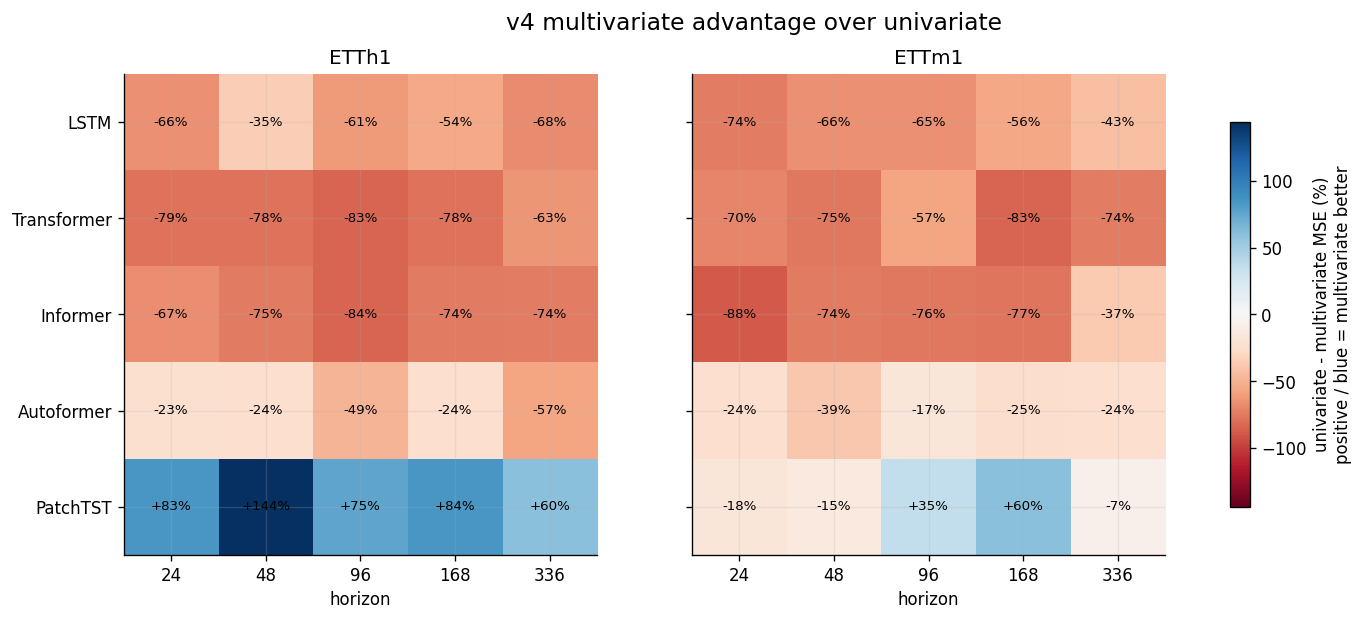
\includegraphics[keepaspectratio]{figures/v4_feature_mode_delta_heatmap.png}}
\caption{v4 单变量/多变量差值热力图}
\end{figure}

这一结果说明，额外变量并不必然改善目标变量预测。对 LSTM、Transformer、Informer 和 Autoformer 而言，单变量模式在当前实验中全部 10 个配对任务上更优，说明多变量输入可能增加学习难度，或使模型更容易受到变量间弱相关、噪声和尺度差异影响。PatchTST 则表现出不同特征：它在 7 个任务中从多变量输入受益，在 3 个任务中单变量更优。这与 PatchTST 的 channel independence 设计相吻合，即模型可以在通道独立建模的基础上较好地利用多变量历史信息，而不是简单地将所有变量混合。

\begin{figure}
\centering
\pandocbounded{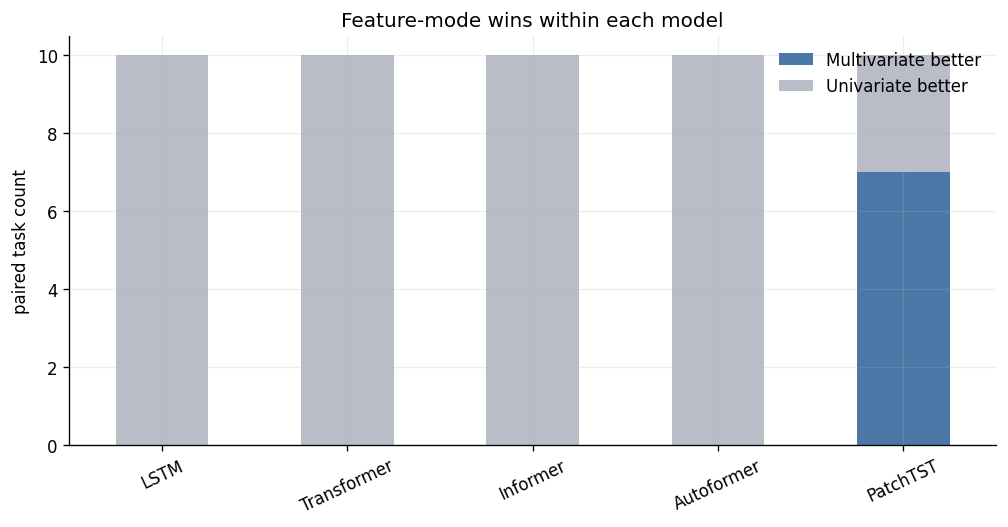
\includegraphics[keepaspectratio]{figures/v4_feature_mode_benefit_counts.png}}
\caption{v4 单/多变量收益次数}
\end{figure}

从 horizon 趋势看，长预测步长下单变量和多变量之间的差异仍然存在，并不会随着预测窗口拉长自然消失。这意味着输入变量选择本身也是长时序预测中的重要设计问题：当模型结构不能有效处理变量间关系时，更多变量可能反而降低目标列预测精度；当模型能够抑制变量间干扰时，多变量信息才更可能转化为有效收益。

\begin{figure}
\centering
\pandocbounded{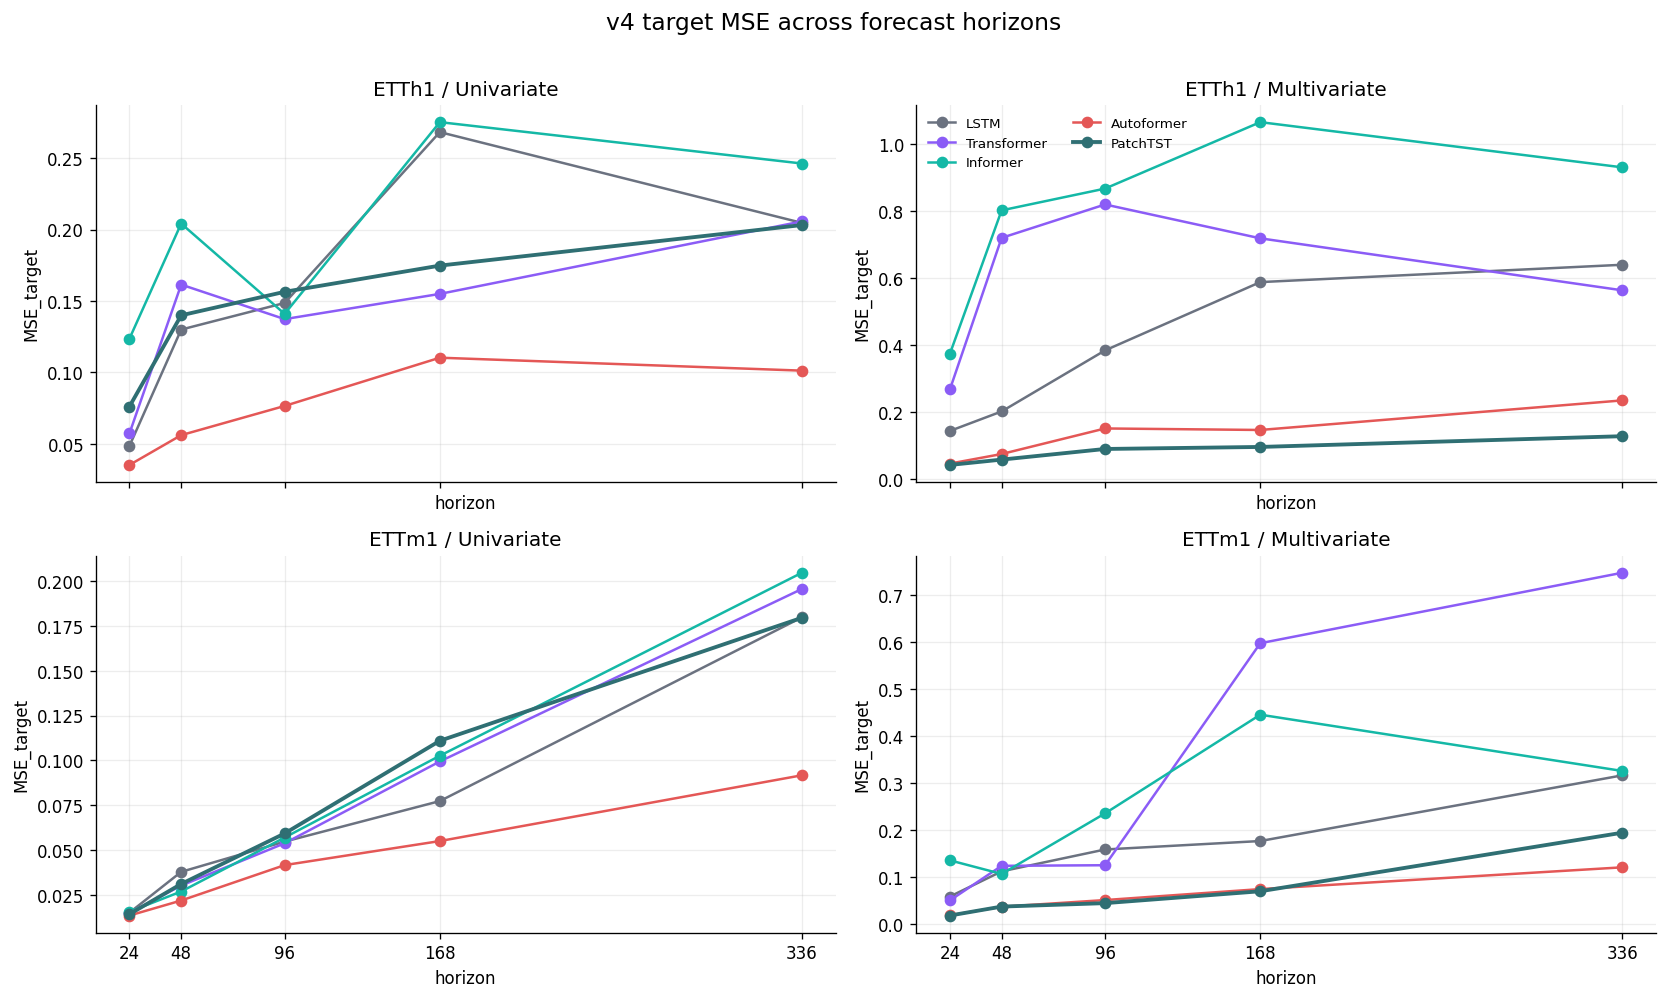
\includegraphics[keepaspectratio]{figures/v4_feature_mode_horizon_trends.png}}
\caption{v4 单/多变量步长趋势}
\end{figure}

\subsection{预测曲线与残差分析}\label{ux9884ux6d4bux66f2ux7ebfux4e0eux6b8bux5deeux5206ux6790}

预测曲线与残差分析是理解长步长预测误差来源的重要方式。理想情况下，本文应基于 v2 最优配置 checkpoint 选取代表性任务，例如 ETTh1 h96 PatchTST、ETTh1 h336 PatchTST、ETTm1 h96 Autoformer 或 PatchTST、ETTm1 h336 Autoformer 或 PatchTST，绘制目标列真实值与预测值曲线，并进一步观察残差随预测步长变化的形态。

不过，当前本地归档的 v2 \texttt{\_results.npy} 文件只保存训练摘要、指标和历史曲线，不包含完整预测序列；本地正式 v2 checkpoint 也不完整，无法在不引入伪结果的情况下重新生成上述代表性预测图。因此，本文在本节保留分析口径而不插入旧 v1 图片。后续补图时应使用 v2 完整 checkpoint 对测试集样本进行推理，优先选择 h96 与 h336 两类预测步长，以便同时观察中期预测和长期预测的差异。

从已有指标趋势仍可推断：随着 horizon 增大，模型整体 MSE 上升、R² 下降，说明远期预测中误差累积更加明显。预测曲线层面通常会表现为输出更平滑、对局部突变反应不足、相位或幅值出现偏差；残差图则可能出现连续偏正或偏负区间，反映模型在某些时间段系统性低估或高估。正式提交前若补齐 v2 预测/残差图，应将图像与这一指标趋势对应起来，而不是只展示单个样本的视觉效果。

\subsection{复杂度与效率分析}\label{ux590dux6742ux5ea6ux4e0eux6548ux7387ux5206ux6790}

模型复杂度不仅体现在参数量上，也体现在训练和推理成本上。v2 主实验中，LSTM 平均参数量约 57.9 万，是五个模型中最高，但平均 MSE 也最高；PatchTST 平均参数量约 11.3 万，平均 MSE 最低。这说明在当前任务中，参数量并不直接决定预测精度，更关键的是结构是否适合时间序列模式。Transformer 的平均参数量约 33.8 万，性能仍弱于 PatchTST 和 Autoformer，也进一步说明标准注意力结构并非天然适合长时序预测。

\begin{figure}
\centering
\pandocbounded{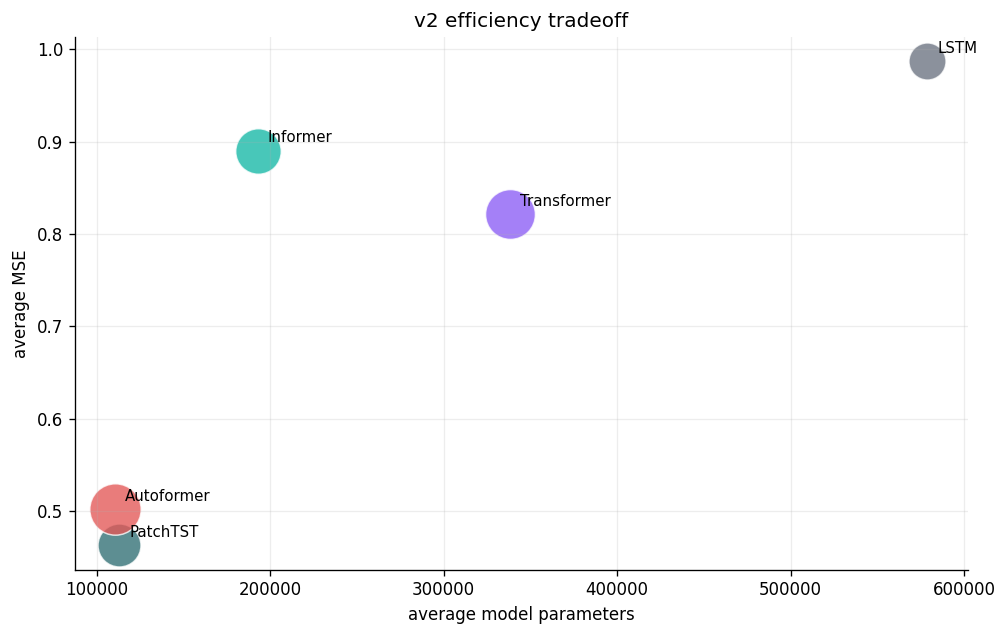
\includegraphics[keepaspectratio]{figures/v2_efficiency_tradeoff.png}}
\caption{v2 效率权衡图}
\end{figure}

训练时间方面，v2 中 LSTM 平均训练时间约 41.1 秒，PatchTST 约 58.7 秒，Informer 约 67.1 秒，Transformer 约 82.6 秒，Autoformer 约 88.3 秒。训练时间受模型结构、early stopping、硬件和实现方式共同影响，因此不应脱离实验环境单独解释。PatchTST 在训练成本相对可控的同时取得最低误差，说明其精度---训练成本权衡较好。

纯 forward 推理时间在本机 Apple MPS 上测得。batch size=1 时，PatchTST 平均中位延迟约 1.3669 ms，Transformer 约 1.4791 ms，LSTM 约 2.2747 ms，Informer 约 2.6577 ms，Autoformer 约 7.2089 ms。batch size=128 时，PatchTST 平均单样本延迟约 0.0416 ms，吞吐量约 24101 samples/s，在五个模型中最高。该结果说明 PatchTST 不仅预测精度较好，纯模型前向计算也较高效。Autoformer 虽然结构解释性强，并且在部分任务中具有较好精度，但 batch size=1 下平均 forward 延迟较高，部署时需要考虑实时性要求。

表 9 给出了纯 forward 推理时间的模型级汇总。batch size=1 更接近单样本实时预测延迟，batch size=128 更适合观察批量推理吞吐。

{\def\LTcaptype{none} % do not increment counter
\begin{longtable}[]{@{}
  >{\raggedright\arraybackslash}p{(\linewidth - 8\tabcolsep) * \real{0.1579}}
  >{\raggedleft\arraybackslash}p{(\linewidth - 8\tabcolsep) * \real{0.2105}}
  >{\raggedleft\arraybackslash}p{(\linewidth - 8\tabcolsep) * \real{0.2105}}
  >{\raggedleft\arraybackslash}p{(\linewidth - 8\tabcolsep) * \real{0.2105}}
  >{\raggedleft\arraybackslash}p{(\linewidth - 8\tabcolsep) * \real{0.2105}}@{}}
\toprule\noalign{}
\begin{minipage}[b]{\linewidth}\raggedright
模型
\end{minipage} & \begin{minipage}[b]{\linewidth}\raggedleft
bs=1 中位延迟/ms
\end{minipage} & \begin{minipage}[b]{\linewidth}\raggedleft
bs=128 中位延迟/ms
\end{minipage} & \begin{minipage}[b]{\linewidth}\raggedleft
bs=128 单样本延迟/ms
\end{minipage} & \begin{minipage}[b]{\linewidth}\raggedleft
bs=128 吞吐/s
\end{minipage} \\
\midrule\noalign{}
\endhead
\bottomrule\noalign{}
\endlastfoot
PatchTST & 1.3669 & 5.3294 & 0.0416 & 24101.4 \\
Transformer & 1.4791 & 15.2688 & 0.1193 & 8395.2 \\
LSTM & 2.2747 & 13.6797 & 0.1069 & 9370.6 \\
Informer & 2.6577 & 32.2407 & 0.2519 & 4029.4 \\
Autoformer & 7.2089 & 15.1731 & 0.1185 & 8506.3 \\
\end{longtable}
}

推理时间的解释必须注意硬件口径：本文推理 benchmark 使用本机 Apple MPS，而 v2 训练结果主要来自 CUDA 环境。二者不能直接用于``同一硬件下训练---推理成本''的严格比较，但可以分别说明训练阶段和部署阶段的成本趋势。若后续需要更严格的工程结论，应在同一 CUDA 机器上复用 \path{scripts/benchmark_inference.py} 重新测量推理时间。

\section{讨论}\label{ux8ba8ux8bba}

第一，长步长预测性能衰减是本文最稳定的现象之一。随着预测步长从 24 增加到 336，模型需要预测更远未来，局部突变和周期相位变化更难提前判断，误差累积随之增强。即使 PatchTST 和 Autoformer 在多数任务中表现较好，也不能完全避免远期预测的不确定性。

第二，模型结构比单纯模型规模更关键。PatchTST 参数量不高，却取得最低平均 MSE 和较优推理效率，说明 patching 和 channel independence 对当前 ETT 数据非常适配。Autoformer 的序列分解消融结果也表明，显式引入趋势/季节结构能显著影响预测表现。相比之下，标准 Transformer 和 LSTM 即使拥有较多参数，也未能取得更好结果。

第三，单变量与多变量预测之间不存在简单的``变量越多越好''。在 50 个配对任务中，单变量模式赢 43 次，说明额外变量可能引入优化负担或噪声。PatchTST 是唯一大量从多变量输入中受益的模型，这说明多变量信息能否转化为预测收益，与模型处理变量间关系的方式高度相关。

第四，本文仍存在局限性。实验数据集只覆盖 ETTh1 和 ETTm1，结论主要反映 ETT 数据在两种采样频率下的相对趋势。正式结果主要基于单随机种子 42，尚未报告多随机种子的均值和方差。当前模型输出为点预测，未进行概率预测或分位数预测；同时，本文的``多变量''指多变量历史序列输入，并未单独引入日历特征、天气变量等外部协变量。因此，本文更适合作为统一实现和统一实验口径下的模型比较，而不是对原论文最优结果的完全复现。

\section{结束语}\label{ux7ed3ux8bed}

本文围绕长时序预测任务，比较了 LSTM、Transformer、Informer、Autoformer 与 PatchTST 五类模型在 ETTh1 和 ETTm1 数据集上的多步预测表现，并通过调参前后对比、消融实验、单变量/多变量对比和推理效率 benchmark 分析模型结构差异。实验结果表明，PatchTST 在 v2 主实验中整体表现最好，跨 10 个数据集---预测步长任务获得 9 次最低 MSE，平均 MSE 为 0.462621；Autoformer 在部分任务中仍有竞争力，平均 MSE 为 0.501605。

消融实验验证了关键结构的重要性：移除 Autoformer 的序列分解模块后，平均 MSE 上升约 66.2\%；取消 PatchTST 的通道独立建模后，平均 MSE 上升约 139.2\%。这说明面向时间序列结构的专门设计对长步长预测具有实质贡献。单变量/多变量对比则表明，额外变量并不必然带来收益，单变量模式在 50 个配对任务中赢得 43 次，而多变量优势全部来自 PatchTST，说明变量利用能力依赖模型结构。

复杂度分析进一步显示，PatchTST 在精度、参数量和纯 forward 推理效率之间具有较好平衡；参数量更大的 LSTM 和 Transformer 并未取得更优结果。总体来看，本文完成了统一数据、统一窗口、统一评价指标下的长时序预测模型比较，能够较清晰地展示不同结构设计对预测精度和计算成本的影响。后续工作可以从三个方向扩展：一是进行多随机种子稳定性实验，报告均值与方差；二是补充概率预测，输出预测区间并评估覆盖率；三是引入外生变量或时间特征，进一步分析外部协变量对长时序预测的作用。

\section*{参考文献}\label{ux53c2ux8003ux6587ux732e}

\begin{thebibliography}{99}
\small
\setlength{\itemsep}{0.2em}

\bibitem{hochreiter1997}
Hochreiter S, Schmidhuber J. Long Short-Term Memory. Neural Computation, 1997, 9(8): 1735--1780.

\bibitem{vaswani2017}
Vaswani A, Shazeer N, Parmar N, et al. Attention Is All You Need. Advances in Neural Information Processing Systems, 2017, 30: 5998--6008.

\bibitem{zhou2021informer}
Zhou H, Zhang S, Peng J, et al. Informer: Beyond Efficient Transformer for Long Sequence Time-Series Forecasting. Proceedings of the AAAI Conference on Artificial Intelligence, 2021, 35(12): 11106--11115.

\bibitem{wu2021autoformer}
Wu H, Xu J, Wang J, Long M. Autoformer: Decomposition Transformers with Auto-Correlation for Long-Term Series Forecasting. Advances in Neural Information Processing Systems, 2021, 34: 22419--22430.

\bibitem{nie2023patchtst}
Nie Y, Nguyen N H, Sinthong P, Kalagnanam J. A Time Series is Worth 64 Words: Long-term Forecasting with Transformers. International Conference on Learning Representations, 2023.

\bibitem{project2026}
涂家俊. 基于 LSTM、Transformer 及其高效变体的长时序预测实验结果与代码. 2026. \path{archive/v2_results/experiments/validation_best_full_matrix/}; \path{archive/v4_results/experiments/ablation_study/}; \path{archive/v4_results/experiments/univariate_multivariate_comparison/}.

\end{thebibliography}

\section*{附录：结果文件与图表清单}\label{ux9644ux5f55ux7ed3ux679cux6587ux4ef6ux4e0eux56feux8868ux6e05ux5355}

\subsection*{A.1 主实验与补充实验表}\label{a.1-ux4e3bux5b9eux9a8cux4e0eux8865ux5145ux5b9eux9a8cux8868}

\begin{itemize}
\tightlist
\item
  v2 主实验汇总：\path{archive/v2_results/experiments/validation_best_full_matrix/summaries/csv/full_val_best_e50p10_tb_seed42_summary.csv}
\item
  v1/v2 调参对比来源：\path{archive/v1_results/experiments/formal_baseline/summaries/csv/formal_seed42_all.csv}
\item
  v4 消融实验汇总：\path{archive/v4_results/experiments/ablation_study/summaries/csv/ablation_rerun_seed42_summary.csv}
\item
  v4 消融配对对比：\path{archive/v4_results/experiments/ablation_study/summaries/csv/ablation_rerun_seed42_comparison.csv}
\item
  v4 单变量/多变量对比：\path{archive/v4_results/experiments/univariate_multivariate_comparison/summaries/csv/feature_mode_full_seed42_comparison.csv}
\item
  v4 单变量/多变量差值表：\path{archive/v4_results/experiments/univariate_multivariate_comparison/summaries/csv/feature_mode_full_seed42_comparison_delta.csv}
\item
  纯 forward 推理时间：\path{archive/v2_results/experiments/validation_best_full_matrix/summaries/csv/pure_forward_inference_benchmark_by_model.csv}
\end{itemize}

\subsection*{A.2 图表清单}\label{a.2-ux56feux8868ux6e05ux5355}

\begin{itemize}
\tightlist
\item
  v2 主实验图：\path{v2_model_average_metrics.png}、\path{v2_horizon_trends.png}、\path{v2_winner_counts.png}
\item
  v1/v2 对比图：\path{v2_vs_v1_model_comparison.png}、\path{v2_vs_v1_task_improvement_heatmap.png}
\item
  v2 效率图：\path{v2_efficiency_tradeoff.png}
\item
  v4 消融图：\path{v4_ablation_mean_effects.png}、\path{v4_ablation_task_delta_heatmap.png}、\path{v4_ablation_resource_tradeoff.png}
\item
  v4 单/多变量图：\path{v4_feature_mode_delta_heatmap.png}、\path{v4_feature_mode_benefit_counts.png}、\path{v4_feature_mode_horizon_trends.png}
\end{itemize}

\subsection*{A.3 推理时间口径}\label{a.3-ux63a8ux7406ux65f6ux95f4ux53e3ux5f84}

推理时间 benchmark 使用 \path{scripts/benchmark_inference.py} 生成，默认覆盖 ETTh1、ETTm1、五个预测步长、五个模型和 batch size 1/128。计时范围仅包含 \path{torch.inference_mode()} 下的 \path{model(x)}，并在 CUDA/MPS 上进行同步；不包含 DataLoader、数据从 CPU 到设备的搬运、反归一化、指标计算或结果写盘。当前结果设备为 Apple MPS。


\end{document}
